\subsection*{Assignment 1.b \hrule}
\textbf{Question}
\begin{quote}
Write a random number generator that returns a random floating-point number between 0 and 1. At minimum, use some combination of an (M)LCG and a 64-bit XOR-shift. Plot a sequential of random numbers against each other in a scatter plot ($x_{i+1}$ vs $x_i$) for the first 100 numbers generated. Additionally, have your code generate 1,000,000 random numbers and plot the result of binning these in 20 bins 0.05 wide. The seed value should be the first output when the code is run.
\end{quote}

\textbf{Solution}
\begin{quote}
To create the random number generator three methods are used. The first two methods are the linear congruential generator (LCG) and a 64-bit XOR-shift. The last method is multiply with carry (MWC). The methods are combined to generate a new seed from the current seed. The new seed is generated by first cloning the current seed and then performing a bitwise xor operation between the XOR-shift method and the LCG method evaluated at the cloned seed. The result is set as the new seed. Next, the result of the MWC method for the cloned seed is subtracted from the new seed. Finally, a bitwise 'and' operation is performed on the new seed to only keep the last 32 bits \footnote{The performed 'and' operation actually changes the number of bits that is used to store the new seed in python. This would not be the case in other languages such as $c++$ or $java$. The performed 'and' operation will in these languages just puts all bits, expect the last 32 bits, to zero.}.  This is done to fix number from becoming 'infinite' large\footnote{Python types can grow as large as possible. Continuous performing bit shifts to the left (i.e continues calling the XOR-shift method)  will therefore result in larger and larger numbers. Eventually the number becomes so large that simple bitwise operation take a significant of time.  }.

The random number generator should only be initialized once and be used in a continues way through out the full assignment. I however splitted each exercise in a small file to make the report look better. The continues usage of the random number generator trough out the full assignment is as result done by initializing it in a new assignment with the final seed of the previous assignment. The code that displays the output will therefore print the seed twice. The first time is the initial seed. The second time is the value of the seed after generating the plots. The value that the seed has the second time is thus used as initial seed in assignment 2.a. 

The code for this assignment is located in two files: \textsf{./code/assignment1\_ b .py} and \textsf{./code/mathlib/rng.py}. The first file contains the code that creates the plots and displays the output. The second file contains the code for the random number generator. The code for both files and the output can be found below.


%that prints the initial seed and creates the plots is \textsf{./code/assigment1\_ b .py}. The code for the random number generator is \textsf{./code/mathlib/rng.py}. The file with the random number generator contains additional functions that are used for the next assignment. The code that displays the output  prints the seed of the random number generator twice. The first time is the initial seed. The second time is the seed after generating the data for the plots.  The random number generator should only be initialized once and be used in a continues way through out the full assignment. I however splitted each exercise in a small file to make the report look better. The continues usage of the random number generator trough out the full assignment is as result done by initializing it in a new question with the final seed of the previous question. The final seed that is printed here is thus used as initial seed in question 2.a.

\end{quote}
\textbf{Code - output } 
\begin{quote}
 The code that produces the output.
\lstinputlisting{./code/assignment1_b.py}
\end{quote}

\textbf{Code - random number generator } 
\begin{quote}
The code for the random number generator. The code contains additional function's that are not used in this exercise, but will be used in the upcoming exercises.
\lstinputlisting{./code/mathlib/rng.py}
\end{quote}


\textbf{Output - Text}
\begin{quote}
The text output produced by \textsf{/code/assignment1\_ b.py} 
\lstinputlisting{./output/assignment1_b_out.txt}
\end{quote}

\textbf{Output - plots}
\begin{quote}
The plots produced by \textsf{/code/assignment1\_ b.py} (see next page).
\newpage
\begin{figure}[!ht]
\centering
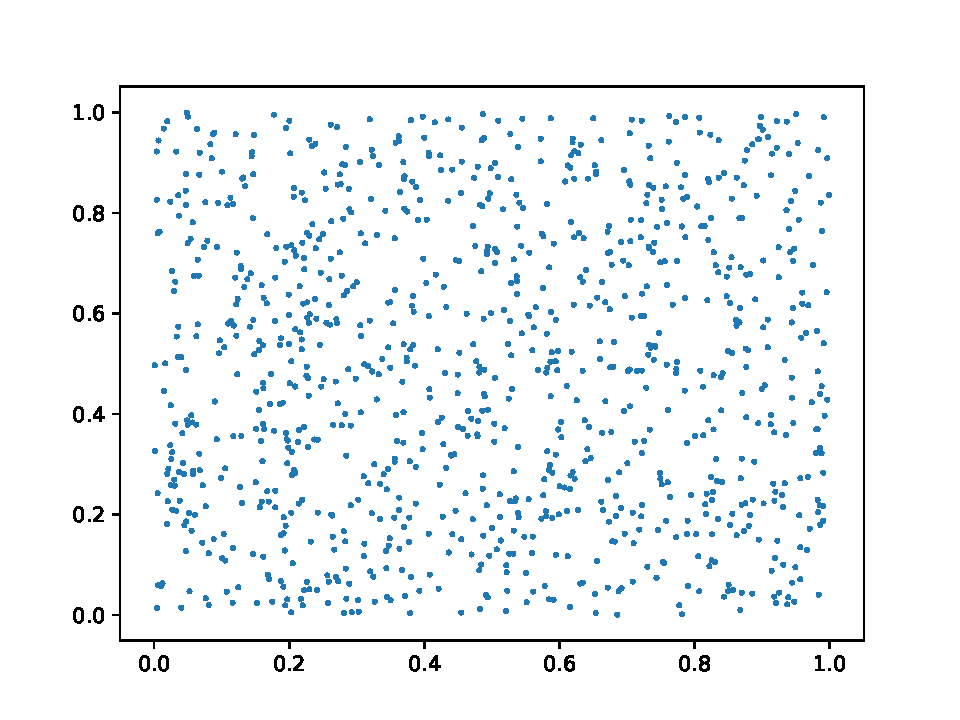
\includegraphics[scale=0.8]{plots/random_next_current.pdf}
\caption{The result of plotting $x_{i+1}$ against $x_i$ for 1000 values. }
\end{figure}
 

\begin{figure}[!hb]
\centering
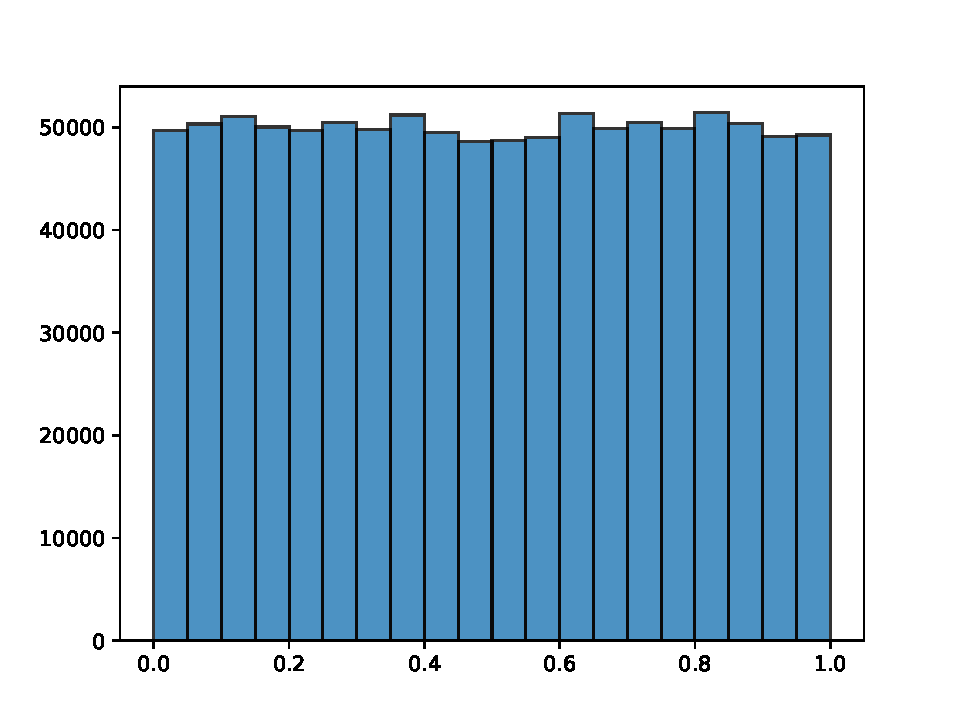
\includegraphics[scale=0.8]{plots/random_uniformness.pdf}
\caption{The uniformness of the random number generator for 1 million generated values between 0 and 1. The values are binned in 20 bins}
\end{figure}
\end{quote}
\newpage
\newpage




%The final output is given by. Here the seed is printed after executing the code as this value will be used for the next exercise (i.e the question was to keep using the same random number generator)
%\lstinputlisting{./assigment1_2_out.txt}








